\documentclass[letterpaper,11pt]{exam}

\usepackage[T1]{fontenc}
\usepackage[top=2cm, bottom=2cm, left=3cm, right=3cm]{geometry}
\usepackage{amssymb}
\usepackage[fleqn]{amsmath} % align equations left
\usepackage{tcolorbox}
\usepackage{xcolor}
\usepackage{xspace}
\usepackage{siunitx} % don't use SIunits!
\usepackage{graphicx}
\DeclareGraphicsExtensions{.pdf,.png,.jpg,.mps,.eps,.ps}
\graphicspath{{figs/}}

\usepackage[numbers,sort&compress,super,comma]{natbib}
\usepackage[framed,numbered]{matlab-prettifier}

\DeclareMathOperator*{\E}{\mathbb{E}} % expectation
\DeclareMathOperator*{\var}{var}
\DeclareMathOperator*{\cov}{cov}
\newcommand{\system}[2]{\mathcal{#1}\left[ #2 \right]}

\newcommand{\iid}{{\it i.i.d.}\xspace}
\newcommand{\iidsample}{\stackrel{iid}{\sim}}
\newcommand{\normalDist}{\mathcal{N}}
\newcommand{\homework}{\textcolor{violet}{\textbf{Homework:}~}}
\newcommand{\funfact}{\textbf{Fun Fact:}~}

\pagestyle{headandfoot}
\runningheadrule
\runningheader{}{Temporal Structure in Neural Data}{Il Memming Park}

\begin{document}
\vspace{-5mm}
\begin{center}
\textbf{\large
    Introduction to temporal structure in neural data
}
\end{center}

In this introductory worksheet, we will deal with discrete time series $x_t$ defined on discrete time indices $t = 0, 1, \ldots$, assuming a periodic sampling scheme.
For example, for voltage measured at \SI{1}{\kilo\hertz} sampling rate, $x_1$ denotes the voltage measured $\Delta = 1/1000 = \SI{1}{\milli\second}$ after $x_0$.
For spike trains, sampling interval of \SI{0.1}{\milli\second} to \SI{1}{\milli\second} range are typically used.

\begin{questions}
\question (Warm up: a linear neuron model)
Let's consider a simple neuron with continuous neural activity (e.g. membrane potential) over time $y_t$, which is linearly related to the stimulus over time $x_t$:
\begin{equation}\label{eq:linearneuron:1}
    y_{t} = a x_{t-1}
\end{equation}
where $a$ is a constant.
\begin{parts}
    \part Let $x_{-1:4} = [0, 1, 0, 2, -1, 0]$, write out the values of $y_{0:5}$, i.e., what are the values of $y_0, y_1, \ldots, y_5$?
    \vspace{\stretch{1}}
    \part Let's say the experimentalist has drawn independent samples from the standard normal distribution at each time point to use as the stimulus $x_t$, i.e.,
    \begin{equation}\label{eq:whitenoise}
	x_t \iidsample \normalDist(0, 1)
    \end{equation}
    for all $t$.
    This is known as the \emph{white noise excitation} which is very useful for studying the response of an unknown system.
    Now that input to the system is random, the response is also random.
    What is the mean of $y_t$, that is, what is the value of $\E[y_t]$?
    \begin{tcolorbox}
	\funfact expectation is linear, specifically, $E[aX] = aE[X]$ for a constant $a$.
    \end{tcolorbox}
    \vspace{\stretch{1}}
    \part Evaluate $\E[x_t y_t]$
    \begin{tcolorbox}
	\funfact if $X$ and $Y$ are independent, $E[XY] = E[X]E[Y]$
    \end{tcolorbox}
    \vspace{\stretch{1}}
    \part Evaluate $\E[x_{t-1} y_t]$
    \vspace{\stretch{1}}
    \part Evaluate $\E[x_{t-2} y_t]$
    \vspace{\stretch{1}}
\end{parts}

\newpage

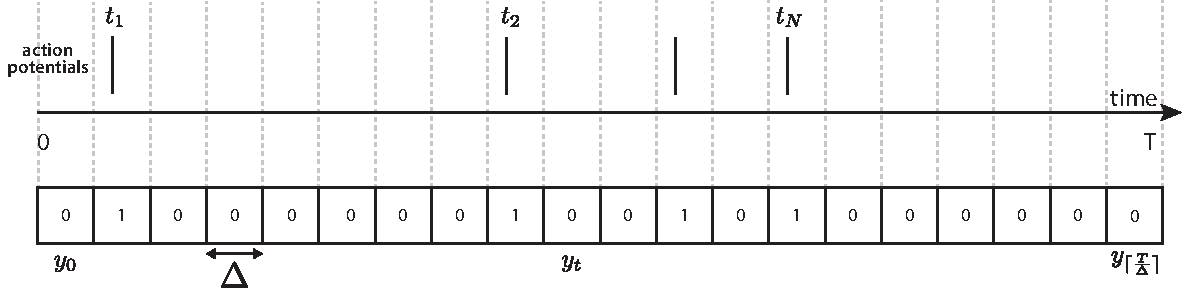
\includegraphics[width=\textwidth]{binned_spike_train}
For a spiking neuron, the neural response is a spike train for which we have two notations to represent them.
Let's consider a time window of $[0, T]$.
First, as an ordered sequence of time points of action potentials, $(0 < t_1 < t_2 < \ldots < t_N < T)$ where there are $N$ action potentials.
Assuming a fixed sampling period $\Delta$, the second representation is as a vector of length $\lceil\frac{T}{\Delta}\rceil$.
Each element of the vector represents a time period, that is $y_t$ corresponds to the time window $[t\Delta, (t+1)\Delta)$.
This vector will have a value of 1 for the time windows that contains an action potential, and 0 for the absence (see illustration above).
This second representation is useful in MATLAB, and called the \emph{binned spike train} in general.
Note that if $\Delta$ is large, there may be more than 1 action potential in the time window, in which case, we store the the number of action potentials in the vector.

\question To characterize the relationship between the stimulus (input) and the spiking response of a neuron (output), we can use \textbf{spike-triggered-average (STA)}:
\begin{tcolorbox}[colback=red!5!white,colframe=red!50!black]
\noindent
\begin{equation}\label{eq:sta}
    \text{STA}(\tau) = \frac{1}{N} \sum_t y_{t} x_{t-\tau}
\end{equation}
\end{tcolorbox}
where $x_t$ is the stimulus, and $y_t$ is the binned spike train.
STA is the average stimulus conditioned on each of the spiking events (non-zero $y_t$).
Larger $\tau$ represents times farther past relative to the triggering spike.
Evaluate the \emph{expected} STA and sketch them for the following neuron models with indepedently random stimulus $x_t$ where $x_t = -1$ with probability $1/2$ and $x_t = 1$ with probability $1/2$.
\begin{parts}
    \part
    \begin{equation}
	y_t = 
	\begin{cases}
	    1 & \text{if $x_{t-1} = 1$}\\
	    0 & \text{otherwise}
	\end{cases}
    \end{equation}
    \begin{tcolorbox}
	\funfact Expectation is linear. $E[X+Y] = E[X] + E[Y]$
    \end{tcolorbox}
    \vspace{\stretch{1}}
\newpage
    \part
    \begin{equation}
	y_t = 
	\begin{cases}
	    1 & \text{if $x_{t-1} = -1$ \textbf{and} $x_{t-2} = 1$}\\
	    0 & \text{otherwise}
	\end{cases}
    \end{equation}
    \vspace{\stretch{1}}
    \part
    \begin{equation}
	y_t = 
	\begin{cases}
	    1 & \text{if $x_{t-1} = -1$ \textbf{or} $x_{t-2} = 1$}\\
	    0 & \text{otherwise}
	\end{cases}
    \end{equation}
    \vspace{\stretch{1}}
\end{parts}

\begin{tcolorbox}
    \funfact STA does not work for an arbitrary stimulus distribution, but it works for white gaussian noise and other elliptically symmetric distributions~\cite{Paninski2003,Park2013f}.
\end{tcolorbox}
We will be analyzing fly visual neuron data from \citet{De_Ruyter_van_Steveninck1997}.
In particular, spikes from the H1 neuron in reponse ($y_t$) to visual motion velocity input ($x_t$) is provided to you.

\question \homework Load the H1 dataset, compute the STA, and plot it.
\textbf{(Instruction: combine all homework answers and submit a single PDF.)}

The result should look something like the plot below.
Note that I have plotted it in reverse time, so that negative lag corresponds to the past.
\begin{figure}[htb]
    \centering
    \includegraphics[width=0.45\textwidth]{data_segment_worksheet}
    \includegraphics[width=0.45\textwidth]{xc_xy}
\end{figure}
\question Explain what you see in the STA figure above.
\begin{parts}
\part Observe that the STA is positive. What does this mean?
    \vspace{\stretch{1}}
\part Observe that the peak and deviation from zero of the STA are on the left of 0 lag. What does this mean?
    \vspace{\stretch{1}}
\part Observe that the rise of the STA peak is fast but decays over \SI{100}{\milli\second}. What does this mean?
    \vspace{\stretch{1}}
\part What kind of neuron model would produce an STA with such a shape?
    \vspace{\stretch{1}}
\end{parts}

\newpage
Before we can discuss nonlinear neuron models, let's consider some linear neurons with internal dynamics, that is the internal state of the neuron influences the time evolution of the neural response. (Unlike our previous linear neuron model which forgot its past instantaneously.)

\question Consider a \textbf{system} (or a filter or a neuron model) that takes an input time series $u_t$, and produces $x_t$. We shall denote such system as: $x_t = \system{H}{u_t}$. In particular, we shall consider a first order recursive model (or filter),
\begin{equation}\label{eq:filter:1}
    x_t = \system{H}{u_t} \triangleq a x_{t-1} + u_t
\end{equation}
where $a$ is a constant.
If you are familiar with conductance based models or leaky-integrate-and-fire neuron model, note their similarity.
\begin{parts}
    \part Let $x_0 = 0$ and $u_t = 0$ for $t \leq 0$.
    Given $u_t$ for $t > 0$, write out the 5 next terms of $x_t$, i.e., what are the values of $x_1, x_2, \ldots, x_5$?
    What's the general expression for $x_t$?
    \vspace{\stretch{1}}
    \part Let $x_0 = 0$ and $u_t = 0$ for all time except at $t=0$, $u_0 = 1$.
    What's the general expression for $x_t$? Sketch them out for $a = 0.5$ and $a = -0.9$.
    \vspace{\stretch{2}}
    \part Show that this system is (1) \textit{linear}, i.e., $\system{H}{\beta u_t} = \beta \system{H}{u_t}$, and (2) \textit{time-invariant}, i.e., $x_t = \system{H}{u_{t}} \implies x_{t+\tau} = \system{H}{u_{t+\tau}}$ for any time shift $\tau$. (\textit{Hint: don't think too much.})
    \vspace{\stretch{2}}
\end{parts}


\newpage

Let's add some noise to the linear time-invariant system.
This provides foundational intuition for temporal data (time series) analysis.

\question Assume a white gaussian noise $\eta_t \sim \mathcal{N}(0, \sigma^2)$ with variance $\sigma^2$.
The \textit{whiteness} comes from being independently drawn at each time step $t$.
Consider the following \textbf{autoregressive process (or model) of order 1}, or \textbf{AR(1)},
\begin{equation}\label{eq:ar1}
    X_t = a X_{t-1} + \eta_t.
\end{equation}
When $|a| < 1$, AR(1) is stationary, that means, for any $n$ and time indices $t_1, \ldots, t_n$, an arbitrary joint expectation shifted in time by $\tau$, $\E[f(X_{t_1+\tau}, X_{t_2+\tau}, \ldots, X_{t_n+\tau})]$ for any function $f$, does not depend on $\tau$.
In other words, you cannot tell $t$ by looking at the random process, since it's always the same kind of random.

\begin{parts}
    \part What is the mean, $\E[X_t]$?
    \vspace{\stretch{1}}
    \part What is the variance, $\var[X_t]$?
\begin{tcolorbox}
    \funfact $\var(aX) = a^2 \var(X)$.
\end{tcolorbox}
\begin{tcolorbox}
    \funfact if $X$ and $Y$ are independent, $E[f(X)g(Y)] = E[f(X)]E[g(Y)]$, also, $\var(X+Y) = \var(X) + \var(Y)$.
\end{tcolorbox}
    \vspace{\stretch{2}}
    \part \homework What is the autocovariance at lag 1, $\cov(X_{t+1}, X_t)$?
    \vspace{\stretch{2}}
\newpage
    \part What is the autocovariance function $\gamma(t, s) = \cov(X_{t}, X_s)$? (\textit{Hint: consider $t \geq s$ case first})?
    \vspace{\stretch{3}}
    \part If $\eta_t$ is actually the external stimulus (measured or generated by the experimentalist), what is the expected STA without the $1/N$ term? (I know, this model doesn't spike.)
    Sketch them out for $a = 0.9$ and $a = -0.5$.
    \vspace{\stretch{3}}
    \part \homework Simulate AR(1) models with $a=0.9$ and $a=-0.9$ and $\sigma=0.01$ for $T=10,000$ time steps. Compute the sample mean and sample variance over time and plot the sample autocorrelation function. Compare these with the theoretical values you derived above. Is the process consistent with being \textit{ergodic}, that is, do the time averages agree with the expectations?
    \part \homework Let $x \triangleq x_{t-1}$ and $y \triangleq x_t$ and observe that \eqref{eq:ar1} is just a straight line with no bias. Simulate an AR(1) model with $a=-0.7$ and $\sigma=0.1$ for $T=10,000$ time steps. Given the time series generated by this AR(1) model, estimate the AR coefficient $a$ using linear regression (least squares).
\end{parts}

\newpage
STA is almost the same as a more widely used quantity, the \emph{cross-correlation function}, which is not restricted to spike trains.
\begin{tcolorbox}[colback=red!5!white,colframe=red!50!black]
\noindent
\begin{equation}
    R_{xy}(t,s) = \E[x_{t}y_s]
\end{equation}
\end{tcolorbox}
If the cross-correlation function only depends on how far the two time points $\tau = t-s$ are, that is, when it is time-invariant (a.k.a. wide-sense stationary), we can simply write:
\begin{equation}
    R_{xy}(\tau) = \E[x_{t+\tau}y_t] = \E[x_t y_{t-\tau}]
\end{equation}
Similarly, \textbf{autocorrelation} is defined as the cross-correlation with itself:
\begin{equation}
    R_{xx}(\tau) = \E[x_{t+\tau}x_t] = \E[x_t x_{t-\tau}]
\end{equation}
\begin{tcolorbox}
    \funfact By the law of large numbers, expectations can be approximated by sample averages.
\end{tcolorbox}
Given $m$ data points over time, we can write an estimator (called the \emph{sample cross-correlation}) as,
\begin{equation}
    \hat{R}_{xy}(\tau) = 
    \begin{cases}
	\frac{1}{m-\tau-1}\sum_{t=0}^{m-\tau-1} x_{t+\tau} y_t & \quad \tau \geq 0\\
	\hat{R}_{xy}(-\tau) & \quad \tau < 0
    \end{cases}
\end{equation}

In MATLAB, the function \texttt{xcorr} computes this without the $\frac{1}{m-\tau-1}$ normalization factor by default (called the \emph{raw} cross-correlation). You can provide extra arguments to choose the desired normalization or scale it appropriately to obtain the STA (with possible lag axis flip).
Try the following MATLAB code:
\lstinputlisting[style=Matlab-Pyglike,basicstyle=\mlttfamily]{code/worksheet_XC.m}

\newpage
\question
From the same H1 dataset, compute the sample autocorrelation function (normalized to correlation coefficients) of the spike train using \texttt{xcorr}. We get the followingn typical shape.
\begin{center}
\includegraphics[width=0.7\textwidth]{ac_y}
\end{center}
\begin{parts}
    \part Why is it symmetric?
    \vspace{\stretch{1}}
    \part Why is the peak at lag $\tau=0$, and why is it $1$?
    \begin{tcolorbox}
	\funfact correlation coefficient is
	\begin{equation}
	    \rho(X,Y) = \frac{\cov(X,Y)}{\sqrt{\var(X)\var(Y)}} \, \in \, [-1, 1]
	\end{equation}
    \end{tcolorbox}
    \vspace{\stretch{1}}
    \part Why is the autocorrelation negative at $\tau=1$?
    \vspace{\stretch{3}}
    \part What does it mean that the autocorrelation approaches 0 at $\tau=50$?
    \vspace{\stretch{3}}
\end{parts}

\newpage

\question
A stationary, finite variance time series can be thought of as the random superposition of sines and cosines oscillating at various frequencies.
Specifically, for such processes, the Fourier transform of the autocovariance function is called the \textbf{power spectral density}, and it captures how much power is captured by each frequency.
\begin{tcolorbox}
    \funfact $e^{2\pi i \omega} = \cos(2\pi\omega) + i \sin(2\pi\omega)$
    (Euler's formula)
    %$a^n = e^{\ln(a)\cdot n}$.
\end{tcolorbox}
\begin{tcolorbox}
    Denote the autocovariance function as $\gamma(\tau) = \cov(X_t, X_{t+\tau})$.
    The power spectral density is defined as:
    \begin{equation}\label{eq:psd:acov}
	f(\omega) \triangleq \sum_{\tau=-\infty}^{\infty} \gamma(\tau) e^{-2\pi i \omega \tau}
    \end{equation}
    The inverse transform is given by,
    \begin{equation}\label{eq:psd:acov:inv}
	\gamma(\tau) = \int_{-1/2}^{1/2} f(\omega) e^{2\pi i \omega \tau} \mathrm{d}\omega
    \end{equation}
    \funfact These are two sides of the same coin!
\end{tcolorbox}
\begin{parts}
    \part What is the power spectral density of white gaussian noise? (\emph{Hint: white gaussian noise is independent gaussian noise with zero mean}.)
    \vspace{\stretch{2}}
    \part \homework Generate $T=10,000$ long white gaussian noise with variance $2$ (i.e., standard deviation $\sqrt{2}$).
    Estimate and plot the power spectral density.
\begin{tcolorbox}
    MATLAB command \texttt{randn} generates ``independent'' gaussian noise with variance $1$.
    MATLAB command \texttt{pwelch} or \texttt{periodogram} can be used to estimate power spectrum given a time series. Try plotting the output!
    \tcblower
    \funfact absolute square of the \texttt{fft} of the raw signal is \underline{not} a (statistically) consistent estimator for the power spectral density. (Don't ever use this method!)
\end{tcolorbox}
\newpage
    \part What is the power spectral density of AR(1) process?
%\vspace*{-8mm}
\begin{align}
    f(\omega) &=
    \sum_{\tau=-\infty}^{\infty} \gamma(\tau) e^{-2\pi i \omega \tau}
    \\
    &= \frac{\sigma^2}{1-a^2} \sum_{\tau=-\infty}^{\infty} a^{|\tau|} e^{-2\pi i \omega \tau}
    \\
    &= \frac{\sigma^2}{1-a^2} \left(
	1 + \sum_{\tau=1}^{\infty} a^{\tau} 
	\left(
	    e^{2\pi i \omega \tau}
	    +
	    e^{-2\pi i \omega \tau}
	\right)
    \right)
    \\
    &= \frac{\sigma^2}{1-a^2} \left(
	1 
	+ \frac{a e^{2\pi i \omega \tau}}{1- e^{2\pi i \omega \tau}}
	+ \frac{a e^{-2\pi i \omega \tau}}{1- e^{-2\pi i \omega \tau}}
    \right)
    \\
    &= \frac{\sigma^2}{1-a^2}
	\frac{1- a e^{2\pi i \omega \tau} a e^{-2\pi i \omega \tau}}
	{(1- a e^{2\pi i \omega \tau})(1- a e^{-2\pi i \omega \tau})}
    \\
    &= \frac{\sigma^2}{1-2a\cos(2\pi\omega)+a^2}\label{eq:ar1:psd}
\end{align}
\part For what range of $a$ values does the AR(1) act as a \textit{low pass filter}, that is, its power spectrum peaks in low frequencies? See below for the plot of~\eqref{eq:ar1:psd}.
\begin{center}
\includegraphics[width=\textwidth]{ar_psd}
\end{center}
    \vspace{\stretch{1}}
    \part \homework Estimate and plot the power spectral density of time series generated from two AR(1) models with parameters of your choice.
\end{parts}

\newpage

\begin{tcolorbox}
    A general order $p$ autoregressive model is,
    \begin{equation}
    X_t \sim \normalDist\left(\sum_{\tau=1}^p a_\tau X_{t-\tau}, \sigma^2\right)
    \end{equation}
\end{tcolorbox}

\question Autoregressive model with order 2, AR(2), can be written as,
\begin{equation}\label{eq:ar2}
    X_t = a_1 X_{t-1} + a_2 X_{t-2} + \eta_t.
\end{equation}
\begin{parts}
    \part Define $\vec{X_t} = 
	\begin{bmatrix}
	    X_t\\
	    X_{t-1}
	\end{bmatrix}$. Rewrite~\eqref{eq:ar2} in matrix-vector form,
	\begin{align}
	    \vec{X_t} = \mathbf{A}\vec{X}_{t-1} + \vec{\eta_t}
	\end{align}

	\begin{align}
	    \mathbf{A} =
	    \begin{bmatrix}
		\qquad,& \qquad\\
		\qquad,& \qquad
	\end{bmatrix}, \qquad
	    \vec{\eta_t} =
	    \begin{bmatrix}
		\qquad &\\
		\qquad &
	    \end{bmatrix}
	\end{align}
\begin{tcolorbox}
    Fun matrix-vector product rule:
    \begin{align}
	\begin{bmatrix}
	    A_{11} & A_{12}\\
	    A_{21} & A_{22}
	\end{bmatrix}
	\begin{bmatrix}
	    x_1\\
	    x_2
	\end{bmatrix}
	=
	\begin{bmatrix}
	    A_{11}x_1 + A_{12}x_2\\
	    A_{21}x_1 + A_{22}x_2
	\end{bmatrix}
    \end{align}
\end{tcolorbox}
    \part \homework In general, when the \textit{eigenvalues} of $\mathbf{A}$ are of magnitude strictly less than 1, the corresponding AR(p) model is stable. Use MATLAB function \texttt{eig} to obtain eigenvalues of a matrix.
    %(These eigenvalues are usually called the roots of the characteristic polynomial in the field of signal processing.)
    Construct a stable AR(2) model by choosing parameters and generate time series of length $T=100,000$. Plot the sample autocorrelation function and estimated power spectral density.
    \part Another way of writing the AR(2) as matrix equations is,
    \begin{align}\label{eq:ar2:row}
	X_t &= \begin{bmatrix} a_1 & a_2 \end{bmatrix}
	\begin{bmatrix}X_{t-1}\\X_{t-2}\end{bmatrix}
	+ \eta_t.
    \end{align}
    Find a way to stack the vectors to write this for all observed data, $x_1, \ldots, x_m$, as one bigger matrix equation. (The new covariate matrix is called the \emph{design matrix}.)
    \begin{align}\label{eq:lsar}
	\begin{bmatrix}
	    x_3\\
	    x_4\\
	    x_5\\
	    \vdots\\
	    x_m
	\end{bmatrix}
	&=
	\begin{bmatrix}
	    \qquad, &\qquad &\\
	    \qquad, &\qquad &\\
	    \qquad, &\qquad &\\
	    \qquad \vdots & &\\
	    \qquad, &\qquad &\\
	\end{bmatrix}
	\begin{bmatrix}
	    \qquad&\\
	    \qquad&
	\end{bmatrix}
	+
	\begin{bmatrix}
	    \qquad &\\
	    \qquad &\\
	    \qquad &\\
	    \quad\vdots &\\
	    \qquad &\\
	\end{bmatrix}
    \end{align}
    \vspace{\stretch{3}}
\newpage
    \part \homework
    Note that above form~\eqref{eq:lsar} is a least squares regression.
    Using the data from Homework 5, estimate the coefficients for the autoregressive model using least squares regression (use the \texttt{/} or \texttt{\textbackslash} command in MATLAB or \texttt{glmfit}).
    Compare the result with the true model parameters.
    \vspace{\stretch{1}}
    \part \homework (optional) A better way of estimating AR model is to use MATLAB functions in the signal processing toolbox: \texttt{aryule, arcov, arberg}. Use each method and compare the result with the true model parameters.
    \vspace{\stretch{1}}
\end{parts}

Note that this is also a \textbf{generalized linear model (GLM)} with Gaussian observation noise.
However, with Gaussian observation noise, we won't get spikes, hence not great for action potentials over time.
To model noisy spiking patterns (a.k.a. point process observations), we can still use GLM but with a Poisson observation noise.
\begin{tcolorbox}[colback=red!5!white,colframe=red!50!black,title=Autoregressive Point Process (a.k.a. Poisson-GLM)]
\noindent
\begin{equation}\label{eq:GLM}
    y_t \sim \text{Poisson}\left(\exp\left( \sum_{\tau=1}^p h_\tau y_{t-\tau} + b\right)\right)
\end{equation}
\end{tcolorbox}
Note the similarity between this GLM formulation (autoregressive point process) and the AR(p) model.

\newpage
\question Consider the GLM in~\eqref{eq:GLM}.
The autoregressive weights $h_\tau$ are called the \emph{history filter} since they dictate how the spiking history impacts the probability of firing now.
\begin{parts}
    \part Recall the absolute refractory period of neurons: Neurons can't fire another action potential within this period. When the time bin size is smaller than the absolute refractory period, what would be the value of $h_1$ that best explains the neural activity?
    \vspace{\stretch{1}}
    \part \homework What is the probability of firing an action potential in the current time bin if there were no spikes for the past $p$ time bins?
    \vspace{\stretch{2}}
    \part What is the log-likelihood of this model?
    \begin{tcolorbox}
	\funfact For a Poisson random variable $y \sim \text{Poisson}(\Lambda)$, its likelihood is,
	\begin{equation}
	    P(y\mid\Lambda) = 
		\frac{\Lambda^y \exp(-\Lambda)}
		{y!}
	\end{equation}
    \end{tcolorbox}
    \vspace{\stretch{4}}
    \part What is the difference in log-likelihood for the homogeneous Poisson model (i.e. GLM with no history filter), and the GLM with $p=1$ if the history filter captured the absolute refractory period per spike? Part of the superior performance of GLMs~\cite{Pillow2008} can be contributed to this.
    \vspace{\stretch{4}}
\end{parts}

\newpage
Do you have other task variables and external stimuli that may drive the neuron you are analyzing\cite{Park2014d}?
\begin{tcolorbox}[colback=red!5!white,colframe=red!50!black,title=GLM with covariates]
\begin{equation}\label{eq:GLM2}
    y_t \sim \text{Poisson}\left(\exp\left( \sum_{\tau=1}^p h_\tau y_{t-\tau} + \sum_{k=1}^K \sum_{\tau=0}^{q_k-1} w^k_\tau x^k_{t-\tau} + b\right)\right)
\end{equation}
where $K$ covariate time series $x^k_t$ are introduced with maximum $q_k-1$ time lags.
\end{tcolorbox}
How do we fit the paprameters of a GLM given spike trains and covariates?
Among many potential estimators, one of the most popular and pricipled estimator is the maximum likelihood estimator (MLE).
In most cases, MLE is \emph{statistically efficient}, that is, the variance of the estimator decays at the fastest possible rate as a function of sample size.
Also, this particular form of MLE has a unique optimal solution, but it may not be the best solution for simulating from the GLM\cite{Arribas2020a}.

In MATLAB, you can use \texttt{glmfit} and \texttt{glmval} to perform MLE-based Poisson regression that can be used to fit our GLM formulations.

\lstinputlisting[style=Matlab-Pyglike,basicstyle=\mlttfamily]{code/worksheet_GLM.m}

Note the logarithm is chosen as the ``link function''. This corresponds to the exponential inverse link function in~\eqref{eq:GLM} and~\eqref{eq:GLM2}.

\newpage
\question (Bonus prep for next lecture) Let $\mathcal{I} = {1, 2, \ldots, n}$ be time indices. The \textbf{covariance matrix} $\Sigma$ is an $n \times n$ real-valued matrix, where each entry is given as $\Sigma_{i,j} = \cov(X_i, X_j)$ for $i, j \in \mathcal{I}$.
\begin{parts}
    \part What are the diagonal entries of $\Sigma$? What would they be if the process is stationary?
    \vspace{\stretch{2}}
    \part If the system is \underline{stationary}, the covariance matrix of the time series has a repeating structure called the \textit{Toeplitz} structure. How many unique values can the covariance matrix have? Are there entries of the second row that are the same as the first row?
    \vspace{\stretch{2}}
    \part Let $\mathbf{X}$ be the data matrix of size $n \times (T-n)$,
    \begin{equation}\label{eq:datamat}
	\mathbf{X} = \begin{bmatrix}
	    X_T       & X_{T-1} & \cdots    & X_{n}
	    \\
	    X_{T-1}   & X_{T-2} & \cdots    & X_{n-1}
	    \\
	    \vdots    & \vdots & \ddots     & \vdots
	    \\
	    X_{T-n+1} & X_{T-n+1} & \cdots  & X_{1}
	\end{bmatrix}
    \end{equation}
    Additionally assume that the observed time series $\mathbf{X}$ has \underline{zero mean}.
    Show that the (biased) \textbf{sample covariance matrix} is given by
    \begin{equation}\label{eq:sample:outer}
	\hat{\Sigma} = \frac{1}{T-n} \mathbf{X}\mathbf{X}^\top
    \end{equation}
    where $(\cdot)^\top$ denotes the \textit{transpose} operation.

	\begin{tcolorbox}
	    Recall the (biased) sample covariance estimator for $\{(X_i, Y_i)\}_{i=1}^{N}$ is,
	\begin{equation}\label{eq:cov:est}
	\cov(X, Y) \approx \frac{1}{N}\sum_i 
	\left(
	    (X_i - \frac{1}{N}\sum_j X_j)
	    (Y_i - \frac{1}{N}\sum_k Y_k)
	\right)
	\end{equation}
	\end{tcolorbox}
    \vspace{\stretch{2}}
\end{parts}
\end{questions}

\nocite{Simoncelli2004}
\nocite{Park2011c}
\nocite{Arribas2020a}
\nocite{Dowling2020a}
\bibliographystyle{plainnat}
\bibliography{refs}
\end{document}
